 \section{Tools}
We used Python as the programming language to implement our code. We chose Python because of it's popularity and easy syntax. There are also a plenty of Pythonn libraries like Tensorflow, Keras and scikit-learn available to easily implement machine learning, deep-learning, natural language processing algorithms. Along with Python as a programming language we also used following programs, tools, and datasets to perform our experiment.
\subsection{HCC}
Due to the high computation requirements for some dataset we needed a faster and reliable hardware. The Holland Computing Center (HCC) claim to be the fastest resource in the state of Nebraska. HCC provides these services to researcher and students associated with any campus of the University of Nebraska system. Some shared services are available for free and dedicated services can be obtained for a modest price. We used their servers to run our Jupyter notebooks.

\subsection{Jupyter Notebook}
Jupyter notebook is part of project Jupyter which aims to provide interactive interface for development across multiple platforms and programming languages. Jupyter's web interface supports data cleaning, data transformation and visualization, numerical operations etc. It allows us to create live code snippets and equations and shows results of inline computation right next to the code in the form of rich media (SVG, LaTeX etc). It combines two components: 
\begin{itemize}
  \item \textbf{A web application}: a web-based interactive tool to write code, markdown, etc. It also displays the rich media output.
  \item \textbf{Notebook documents}: a representation of all the content written and displayed using the web application.
\end{itemize}
Jupyter notebook is gaining rapid popularity in the field of data science for making sharing documentation and codes for replication very easy. In this project, the codes are written in python notebook which can be accessed from our github repository.

\subsection{Tensorflow}
TensorFlow is an end-to-end open source platform for machine learning. It has a comprehensive, flexible ecosystem of tools, libraries and community resources that lets researchers push the state-of-the-art in ML and developers easily build and deploy ML powered applications
TensorFlow\textsuperscript{TM} is an open source software library developed within Google’s AI organization by the Google Brain team with a strong support for machine learning and deep learning. Its flexible architecture allows easy deployment of computation across a variety of platforms (CPUs, GPUs, TPUs), and from desktops to clusters of servers to mobile and edge devices. It is being used at a number of well known companies like Uber, Google, AMD, etc. for high performance numerical computation and machine learning. While TensorFlow is capable of handling a wide range of tasks, it is mainly designed for deep neural network models. It will serve as baseline to test the metamorphic relations identified in section \ref{MRused}. Tensorflow provides api for loading the MNIST dataset identified in section \ref{dataset}. We also used tensorflow to implement neural network and convolutional neural network defined in section \ref{Algorithms}

\subsection{Scikit-learn}
Scikit-learn is a Python module for machine learning built on top of SciPy and is distributed under the 3-Clause BSD license.
It provides a range of supervised and unsupervised learning algorithms via a consistent interface in Python.


\section{Algorithms}\label{Algorithms}
We implemented some popular machine learning algorithms to test our hypothesis that "small changes to input data will not affect the accuracy of the model drastically". We used TensorFlow and scikit-learn to implement the machine learning algorithms. 
\subsection{Convolutional neural network}
The images in the MNIST dataset is a one dimensional vector of 784 features (28x28 pixels). We first reshape the images to match the picture format height x width x channel. Each image in the MNIST dataset is now a single-channel of 28x28x1 size. The images are now fed into the network as input. The first convolution layer has 32 filters with a kernel size of five. The activation function we used is the ReLU function and the output from this layer is fed into a pooling layer. The data goes through another iteration of convolution and pooling before being flattened and sent to the fully connected layer. The output layer gives us a number which corresponds to the class of the image it is assigned to.

\subsection{Neural network}



 Hidden fully connected layer with 256 neurons. Each hidden layer is made up of a set of neurons, where each neuron is fully connected to all neurons in the previous layer, and where neurons in a single layer function completely independently and do not share any connections. If the image is a 64 by 64 greyscale image, then we'd have 64x64=4,096 input neurons, with the intensities scaled appropriately between 0 and 1. The output layer will contain just a single neuron, with output values of less than 0.5 indicating "input image is not a 9", and values greater than 0.5 indicating "input image is a 9 ". The input pixels are greyscale, with a value of 0.0 representing white, a value of 1.0 representing black, and in between values representing gradually darkening shades of grey. The second layer of the network is a hidden layer.

2 layer


\subsection{Naive Bayes}
We used scikit-learn to implement Naive Bayes algorithm. The images were first transformed to a one dimensional vector of 784 features. 
A naive bayes classifier is then created using the $sklearn.naive\_bayes.MultinomialNB()$ function. This classifier is then fitted using the $fit()$ function, which takes the images and labels as input and fits the classifier according to the images and labels. The resulting classifier is then used to predict the labels of test data.

\subsection{$k$-Nearest Neighbor}
 We used scikit-learn to implement our $k$-nearest neighbor algorithm. Scikit's $sklearn.neighbors$ module provides functionality for unsupervised and supervised neighbors-based learning methods. 
 The $KNeighborsClassifier$ function from the $sklearn.neighbors$ module implements learning based on the $k$ nearest neighbors of each query point, where $k$ is an integer value specified by the user. The $k$-neighbors classification in KNeighborsClassifier is the most commonly used technique. Since the optimal value $k$ is dependent on data we ran the experiment with multiple values of $k$ and found that the $k$=3 produces the best accuracy. In general a larger $k$ suppresses the effects of noise, but makes the classification boundaries less distinct.
 We used Euclidean distance as the distance metric and assigned equal weights to all the query points. In some cases it might be better to assign weights based on the distance. The close query point contribute more to the fit and the ones far contribute less. For our case the uniform weight with simple majority vote of the nearest neighbors worked just fine.

\subsection{SVM}
Our support vector machine algorithm was also implemented using scikit-learn. The $sklearn.svm.SVC$ class is based on libsvm and is capable of performing multi-class classification. Internally, they use libsvm and liblinear to handle all computations. These libraries are wrapped using C and Cython. It supports multi-class classification on a one-vs-one scheme. In this scheme a classifier is created for each pair of classes and during prediction, the class which receives most votes is assigned to the data point. In an event of a tie, the class with highest total confidence calculated by summing over the pair-wise classification confidence is selected. 
As the other classifiers, $skleran.SVM$ also takes as input two arrays: an array of training samples and another array of class labels. The training samples and labels are first sent to $fit$ function which fits the SVM model according to the data. The resulting model is then used to predict the labels of test data. 

\section{Dataset}\label{dataset}
To have a variety of dataset we selected the following three datasets for our experiment.
Many experiments are data dependent. To see if our technique is not data dependent we used three different datasets.
\subsection{MNIST Dataset}
The MNIST database of handwritten digits maintained by Yann LeCun \cite{MNIST}, has a training set of 55,000 examples, and a test set of 10,000 examples. It is a subset of a larger set available from NIST. The digits have been size-normalized and centered in a fixed-size image. It is a good database for people who want to try learning techniques and pattern recognition methods on real-world data while spending minimal efforts on preprocessing and formatting. The MNIST database was constructed from NIST's Special Database 3 and Special Database 1 which contain binary images of handwritten digits. The original black and white (bilevel) images from NIST were size normalized to fit in a 20x20 pixel box while preserving their aspect ratio. The images were centered in a 28x28 image by computing the center of mass of the pixels, and translating the image so as to position this point at the center of the 28x28 field.

\subsection{EMNIST Dataset}
The EMNIST dataset is a set of handwritten character digits derived from the NIST Special Database 19
and converted to a 28x28 pixel image format. The EMNIST dataset structure directly matches the MNIST dataset.

\subsubsection{Dataset Summary}
There are six different splits provided in this dataset. A short summary of the dataset is provided below:
\begin{itemize}
  \item EMNIST ByClass: 814,255 characters. 62 unbalanced classes.
  \item EMNIST ByMerge: 814,255 characters. 47 unbalanced classes.
  \item EMNIST Balanced:  131,600 characters. 47 balanced classes.
  \item EMNIST Letters: 145,600 characters. 26 balanced classes.
  \item EMNIST Digits: 280,000 characters. 10 balanced classes.
  \item EMNIST MNIST: 65,000 characters. 10 balanced classes.
\end{itemize}
The full complement of the NIST Special Database 19 is available in the ByClass and ByMerge splits. The EMNIST Balanced dataset contains a set of characters with an equal number of samples per class.
The EMNIST Letters dataset merges a balanced set of the uppercase and lowercase letters into a single 26-class task. The EMNIST Digits and EMNIST MNIST dataset provide balanced handwritten digit datasets directly compatible with the original MNIST dataset.

\begin{figure}[htb!]
        \centering
        \begin{subfigure}[b]{\textwidth}
            \centering
            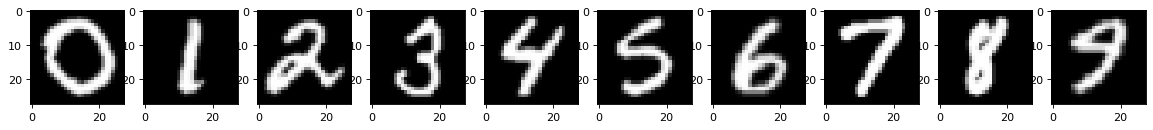
\includegraphics[width=\linewidth]{images/digit.png}
            \caption{Sample EMNIST-MNIST dataset}
            \label{fig:EMNIST MNIST dataset}
        \end{subfigure}%
        \label{fig:Rotate-misclassifications}
        \begin{subfigure}[b]{\textwidth}
            \centering
            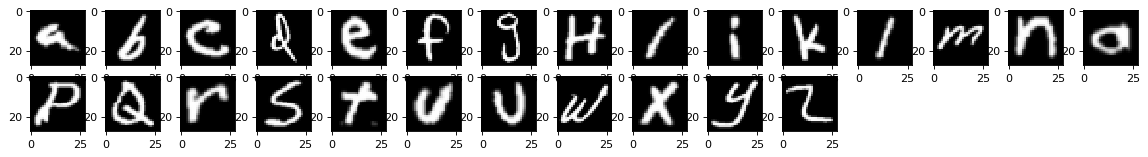
\includegraphics[width=\linewidth]{images/letter.png}
            \caption{Sample EMNIST-Letter dataset}
            \label{fig:EMNIST MNIST dataset}
        \end{subfigure}%
        \label{fig:Rotate-misclassifications}
    \end{figure}
    \FloatBarrier

    
\subsection{Fashion MNIST Dataset}
Fashion-MNIST is a dataset of Zalando's article images-consisting of a training set of 55,000 examples and a test set of 10,000 examples. Each example is a 28x28 grayscale image, associated with a label from 10 classes. 

\begin{table}[ht]
\centering
\begin{tabular}{|c|c|}
\hline
\textbf{Label} & \textbf{Description} \\ \hline
0  &   T-shirt/top \\ \hline
1  &   Trouser \\ \hline
2   &	Pullover \\ \hline
3   &	Dress \\ \hline
4   &	Coat \\ \hline
5   &	Sandal \\ \hline
6   &	Shirt \\ \hline
7   &	Sneaker \\ \hline
8   &	Bag \\ \hline
9   &	Ankle boot \\ \hline
\end{tabular}
\caption{Data file format.}
\label{tbl:training-file-format}
\end{table}

\begin{figure}[htb!]
        \centering
        \begin{subfigure}[b]{\textwidth}
            \centering
            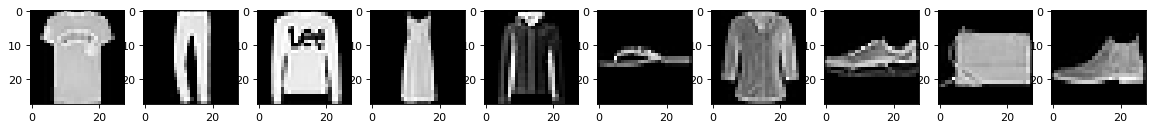
\includegraphics[width=\linewidth]{images/fashion.png}
            \caption{Sample EMNIST-MNIST dataset}
            \label{fig:EMNIST MNIST dataset}
        \end{subfigure}%
        \label{fig:Rotate-misclassifications}
    \end{figure}
    \FloatBarrier
    
\subsection{Format of Dataset}
The data is stored in a very simple file format designed for storing vectors and multidimensional matrices. All the integers in the files are stored in the MSB first (high endian) format used by most non-Intel processors. There are 4 files:
\begin{itemize}
  \item train-images-idx3-ubyte: training set images
  \item train-labels-idx1-ubyte: training set labels
  \item t10k-images-idx3-ubyte:  test set images
  \item t10k-labels-idx1-ubyte:  test set labels
\end{itemize}
The format of training and test files are described in the following table.
\begin{table}[ht]
\centering
\begin{tabular}{|c|c|c|c|}
\hline
\textbf{offset} & \textbf{type}    &      \textbf{value}    &      \textbf{description} \\
\hline
0000  &   32 bit integer & 0x00000801(2049) & magic number (MSB first) \\
\hline
0004  &   32 bit integer & 60000       &     number of items \\
\hline
0008  &   unsigned byte  & ??          &     label \\
\hline
0009  &   unsigned byte  & ??          &     label \\
\hline
\multicolumn{4}{|c|}{\textbf{........}} \\
\hline
xxxx  &   unsigned byte  & ??          &     label \\
\hline
\multicolumn{4}{|c|}{\textbf{The label values are 0 to 9.}} \\
\hline
\end{tabular}
\caption{Training data file format.}
\label{tbl:training-file-format}
\end{table}

\begin{table}[ht]
\centering
\begin{tabular}{|c|c|c|c|}
\hline
\textbf{offset} & \textbf{type}    &      \textbf{value}    &      \textbf{description} \\
\hline
0000  &   32 bit integer & 0x00000803(2051) & magic number (MSB first) \\
\hline
0004  &   32 bit integer & 60000       &     number of images \\
\hline
0008  &   unsigned byte  & 28          &     number of rows  \\
\hline
0012  &   unsigned byte  & 28          &     number of columns \\
\hline
0016  &   unsigned byte  & ??          &     pixel \\
\hline
0017  &   unsigned byte  & ??          &     pixel \\
\hline
\multicolumn{4}{|c|}{\textbf{........}} \\
\hline
xxxx  &   unsigned byte  & ??          &     pixel \\
\hline
\multicolumn{4}{|c|}{\textbf{
\shortstack{Pixels are organized row-wise. Pixel values are 0 to 255. \\ 0 means background (white), 255 means foreground (black).}}} \\
\hline
\end{tabular}
\caption{Test data file format.}
\label{tbl:test-file-format}
\end{table}



% \subsection{Docker}
% For replication of results. Image can be downloaded from dockerhub. Attached volume for persisting data.


